\documentclass[xcolor=dvipsnames,10pt,aspectratio=169]{beamer}
%\usetheme[hideallsubsections]{Hannover}
\usetheme[width=1.9cm]{Hannover} % plenty of themes to pick from
\usefonttheme[onlymath]{serif}
\graphicspath{{../../images/}}
\usepackage[utf8]{inputenc}
\usepackage[T1]{fontenc}
\usepackage{amsmath}
\usepackage{amsfonts}
\usepackage{amssymb}
\usepackage{braket}
\usepackage{bm}
\usepackage{textpos}
\usepackage{multicol}
\usepackage{graphicx,hyperref,url}
\usepackage{tikz}
\usepackage{verbatim}
\usepackage{pgfplots}
\usetikzlibrary{arrows,shapes}
\usecolortheme{crane} % plenty of color themes to pick from
\useinnertheme{rectangles}

\definecolor{UBCgreen}{RGB}{30, 77, 43} % UBC Blue (primary)
\definecolor{UBCgold}{RGB}{200, 195, 114} % UBC Grey (secondary)

\setbeamertemplate{caption}{\raggedright\insertcaption\par}
\setbeamercolor{palette primary}{bg=UBCgreen,fg=white}
\setbeamercolor{palette secondary}{bg=UBCgreen,fg=white}
\setbeamercolor{palette tertiary}{bg=UBCgreen,fg=white}
\setbeamercolor{palette quaternary}{bg=UBCgreen,fg=white}
\setbeamercolor{palette sidebar primary}{fg=black,bg=UBCgold}
\setbeamercolor{palette sidebar secondary}{fg=black,bg=UBCgold}
\setbeamercolor{palette sidebar tertiary}{fg=black,bg=UBCgold}
\setbeamercolor{palette sidebar quaternary}{fg=black,bg=UBCgold}
\setbeamercolor{structure}{fg=UBCgreen} % itemize, enumerate, etc
\setbeamercolor{section in toc}{fg=UBCgreen} % TOC sections
\setbeamercolor{subsection in head/foot}{bg=UBCgold,fg=white}
\setbeamercolor{section in sidebar}{fg=UBCgreen}
\setbeamercolor{section in sidebar}{fg=UBCgreen}
\setbeamerfont{section in sidebar}{size=\small}
\setbeamerfont{title in sidebar}{size=\tiny}
\setbeamerfont{author in sidebar}{size=\tiny}
\setbeamertemplate{page number in head/foot}[appendixframenumber]
\setbeamertemplate{navigation symbols}{\footnotesize\usebeamertemplate{page number in head/foot}}
\setbeamertemplate{frametitle}[default][left,colsep=-4bp,rounded=false]
\setbeamertemplate{section in toc}[bullets]
\addtobeamertemplate{title page}{}{%
    \begin{textblock*}{100mm}(0.445\textwidth,-21.4em)
      
\includegraphics[width=1.5cm]{./figures/CSU-Ram-357-617.png}
    \end{textblock*}
}
\addtobeamertemplate{frametitle}{}{%
    \begin{textblock*}{100mm}(0.95\textwidth,-0.95cm)
      
\includegraphics[width=0.925cm]{./figures/CSU-Ram-357-617.png}
    \end{textblock*}
}
\makeatletter
\setbeamertemplate{sidebar canvas \beamer@sidebarside}%
                  [vertical shading][top=UBCgold,bottom=UBCgold]
\makeatother

%\addtobeamertemplate{sidebar left}{}{
%  \hspace{0.3cm}
%  \vspace{0.2cm}
%  
\includegraphics[align = l, width = 1cm]{CSU-Ram-357-617.pdf}
%}

%\setbeamertemplate{section in toc}{\hspace*{0em}\inserttocsection}
%\setbeamertemplate{subsection in toc}{\hspace*{2em}\inserttocsubsection}

\let\oldhat\hat
\renewcommand{\hat}[1]{\oldhat{\mathbf{#1}}}
\renewcommand{\vec}[1]{\mathbf{#1}}

\newcommand{\ham}{\mathcal{H}}
\newcommand{\ke}{k_{\epsilon}}
\newcommand{\kpm}{k_{\pm}}
\newcommand{\sx}{\sigma_x}
\newcommand{\sy}{\sigma_y}
\newcommand{\sz}{\sigma_z}
\newcommand{\so}{\sigma_0}
\newcommand{\cc}{c^{\dagger}}
\newcommand{\de}{\Delta}

\newcommand{\TT}{Superconducting Triangular Islands as a Platform for Manipulating Majorana Zero Modes}
\newcommand{\ST}{Superconducting triangular islands as a platform for manipulating Majorana zero modes}
\newcommand{\MO}{Motivation}
\newcommand{\KT}{Kitaev Triangle}
\newcommand{\HT}{Hollow Triangle}
\newcommand{\BR}{Braiding}
\newcommand{\CO}{Summary}

\title[\ST]{\TT}
\subtitle{}
\author[Aidan Winblad]{Aidan Winblad \small \and\\ Hua Chen}
\institute{Department of Physics \and\\ Colorado State University}
\date{\small March 8, 2024}

\begin{document}

  \begin{frame}
  \titlepage
  \end{frame}

%  \begin{frame}
%  \frametitle{Outline}
%    \begin{itemize}
%      \item \MO:
%        \begin{itemize}
%          \item P-wave superconductors and braiding
%          \item 1D wires and T-junctions
%          \item Triangular structures for braiding
%        \end{itemize}
%      \item \FO:
%        \begin{itemize}
%          \item Prior results
%          \item Peierls substitution in Kitaev's model
%        \end{itemize}
%      \item \RE:
%        \begin{itemize}
%          \item Topological phase
%          \item Triangular chain
%          \item Hollow triangles
%        \end{itemize}
%      \item \CO
%    \end{itemize}
%  \end{frame}

  \section{\MO}
  \begin{frame}{\MO}{}

    \begin{multicols}{2}

    \begin{itemize}
      \item P-wave superconductors contain half-quantum vortices.
        \begin{itemize}
          \item Majorana fermions located at core of a vortex.
          \item Braiding vortices exhibits Non-Abelian statistics.
        \end{itemize}
      \item 1D p-wave superconductors host Majorana fermions on end points.
        \begin{itemize}
          \item Measurements in real systems:
          \item[] \hspace{0.40em}\scriptsize V. Mourik, \textit{Science} \textbf{336}, 1003 (2012)
          \item[] \hspace{0.50em}\scriptsize S. Nadj-Perge, \textit{Science} \textbf{346}, 602 (2014)
          \item[] \hspace{0.50em}\scriptsize L. Schneider, \textit{Nat. Nanotechnol.} \textbf{17}, 384 (2022)
        \end{itemize}
      \item Quasi-1D T-junction
        \begin{itemize}
          \item Braiding of Majorana fermions is defined for 2D.
          \item In practice challenging to make, but still feasible and seriously pursued.
        \end{itemize}
    \end{itemize}

    \begin{figure}
      \begin{tikzpicture}
        \node[inner sep=0pt] (figure) at (0,0)
        {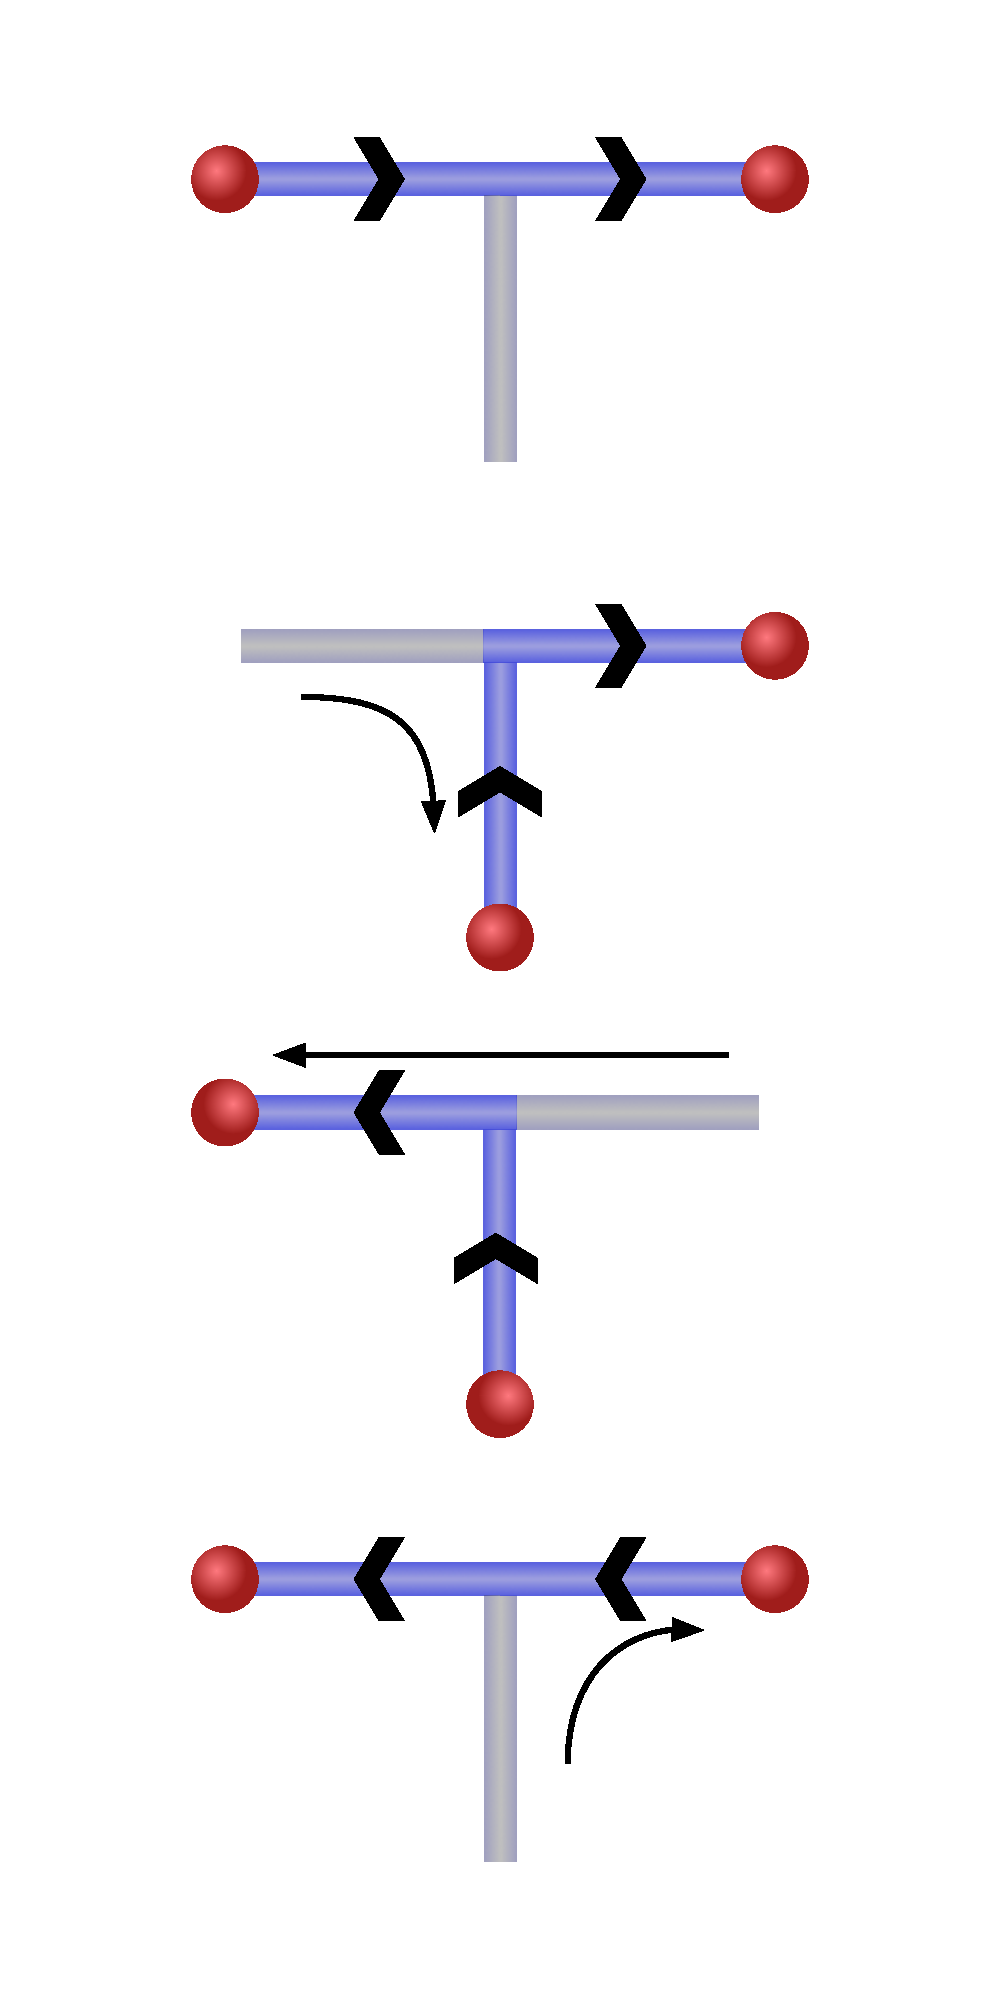
\includegraphics[width=0.25\textwidth]{./figures/t-junction.pdf}};
        \node[inner sep=0pt] (reference) at (0,-3.2) {\small Alicea, \textit{Nature Phys.} \textbf{7}, 412 (2011)}
        \end{tikzpicture}
      \end{figure}
    \end{multicols}

  \end{frame}

  \begin{frame}
    \frametitle{\MO}
    \begin{multicols}{2}

    \begin{itemize}
      \item Consider triangular islands, topologically similar to T-junctions.
      \item Islands of three-fold rotational symmetry occur naturally in epitaxial growth on close-packed metal surfaces.
      \item Good platform for transition from 2D to 1D topological superconductor.
    \end{itemize}
    \newline

    \begin{figure}
      \begin{tikzpicture}
        \node[inner sep=0pt] (figure) at (0,0)
        {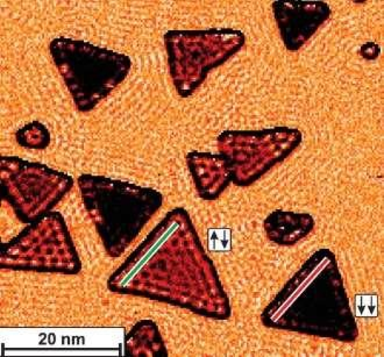
\includegraphics[width=0.4\textwidth]{./figures/triangular-islands.pdf}};
        \node[inner sep=0pt] (caption) at (0,-2.8) {\scriptsize Triangular Co islands on Cu(111).};
        \node[inner sep=0pt] (reference) at (0,-3.2) {\small Pietzsch et al., \textit{PRL} \textbf{96}, 237203 (2006)}
        \end{tikzpicture}
      \end{figure}
    \end{multicols}

  \end{frame}


  \section{\KT}

  \begin{frame}
    \frametitle{Kitaev Triangle}


    \begin{multicols}{2}
      \footnotesize
      \begin{equation*}
        \ham = \sum_{\langle j,l\rangle} \left[ -t e^{i\phi_{jl}}\cc_{j} c_l + \de e^{i\theta_{jl}} c_{j}c_l + h.c.\right] - \sum_j \mu \cc_j c_j
      \end{equation*}

      \vspace{-05mm}
      \begin{figure}
        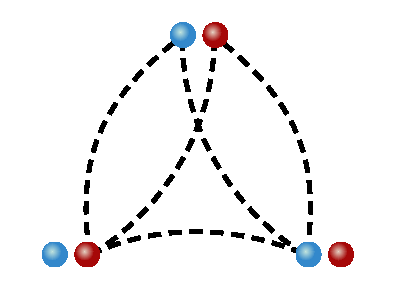
\includegraphics[width=.3\textwidth]{./figures/3-point-triangle.pdf}
      \end{figure}

      \vspace{-05mm}
      \footnotesize
      \begin{align*}
        (\phi_{12},\phi_{23},\phi_{31}) &= \left(0, -\dfrac{\pi}{3}, -\dfrac{\pi}{3}\right) = \bm\phi_1 \\
        &\rightarrow \left( -\dfrac{\pi}{3}, -\dfrac{\pi}{3}, 0 \right) = \bm\phi_2 \\
        &\rightarrow \left( -\dfrac{\pi}{3}, 0, -\dfrac{\pi}{3} \right) = \bm\phi_3 \\
        &\rightarrow \bm\phi_1
      \end{align*}

      \pause
      \begin{figure}
        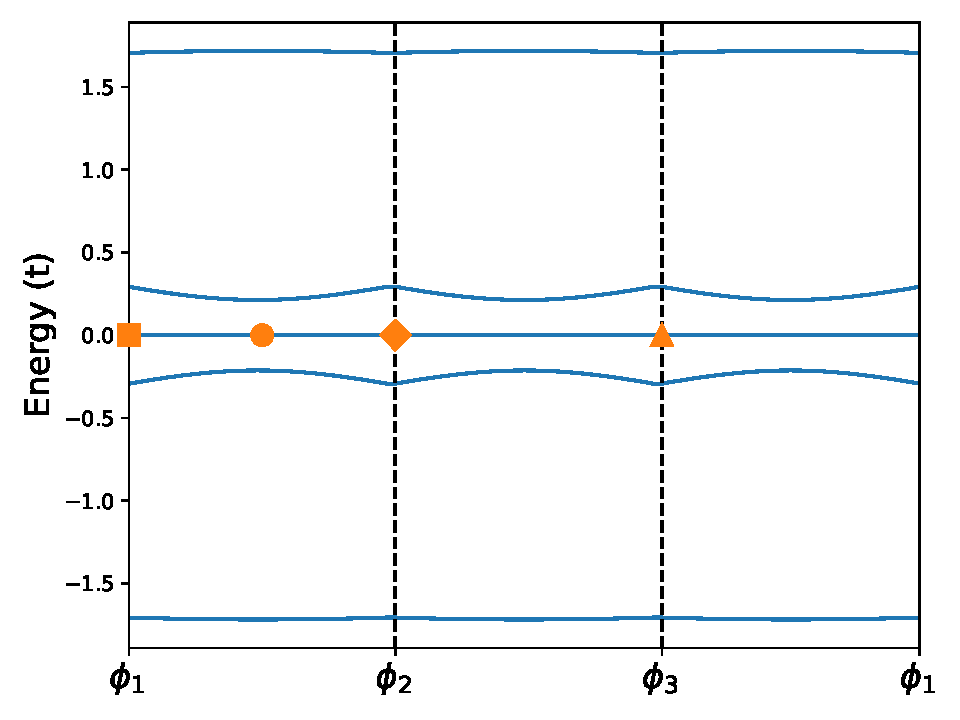
\includegraphics[width=15em]{./figures/3eigval.pdf} \\
        \hspace{3mm}
        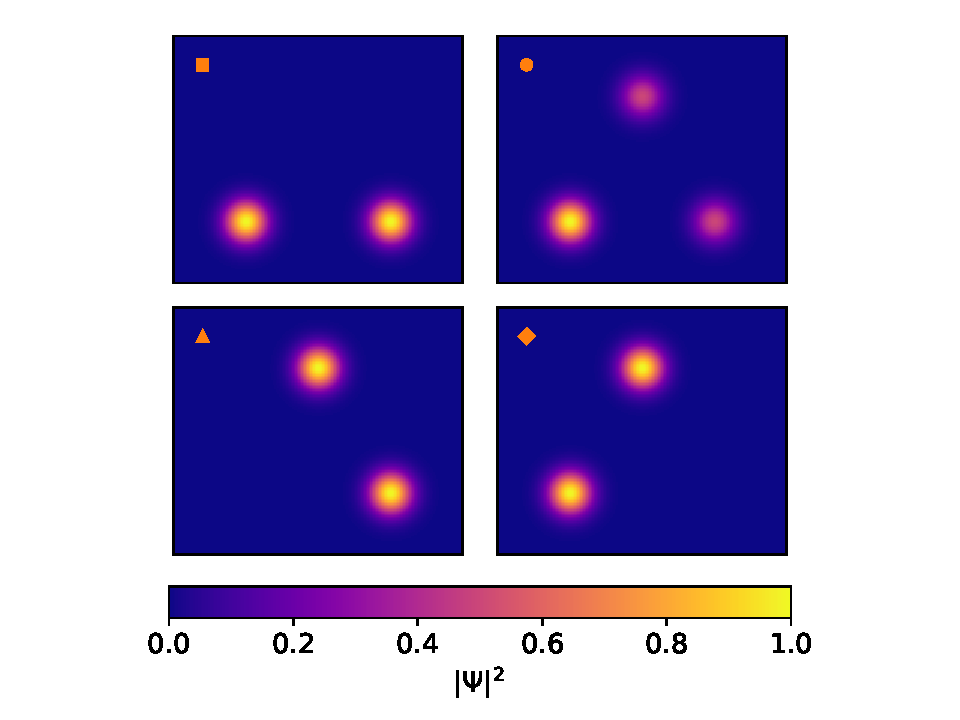
\includegraphics[width=17em]{./figures/3eigvec.pdf}
      \end{figure}

    \end{multicols}

  \end{frame}

  \section{\HT}

  \begin{frame}
    \frametitle{Triangular Ribbon and Topological Phases}
    % show spectral plot and wavefunction

    \begin{multicols}{2}
      \small
      \begin{equation*}
        \phi_{jl} = \dfrac{e}{\hbar}\int_{\vec{r}_j}^{\vec{r}_l} \vec{A} \cdot d\vec{l} = -\phi_{lj}
      \end{equation*}
      \vspace{-08mm}
      \begin{figure}
        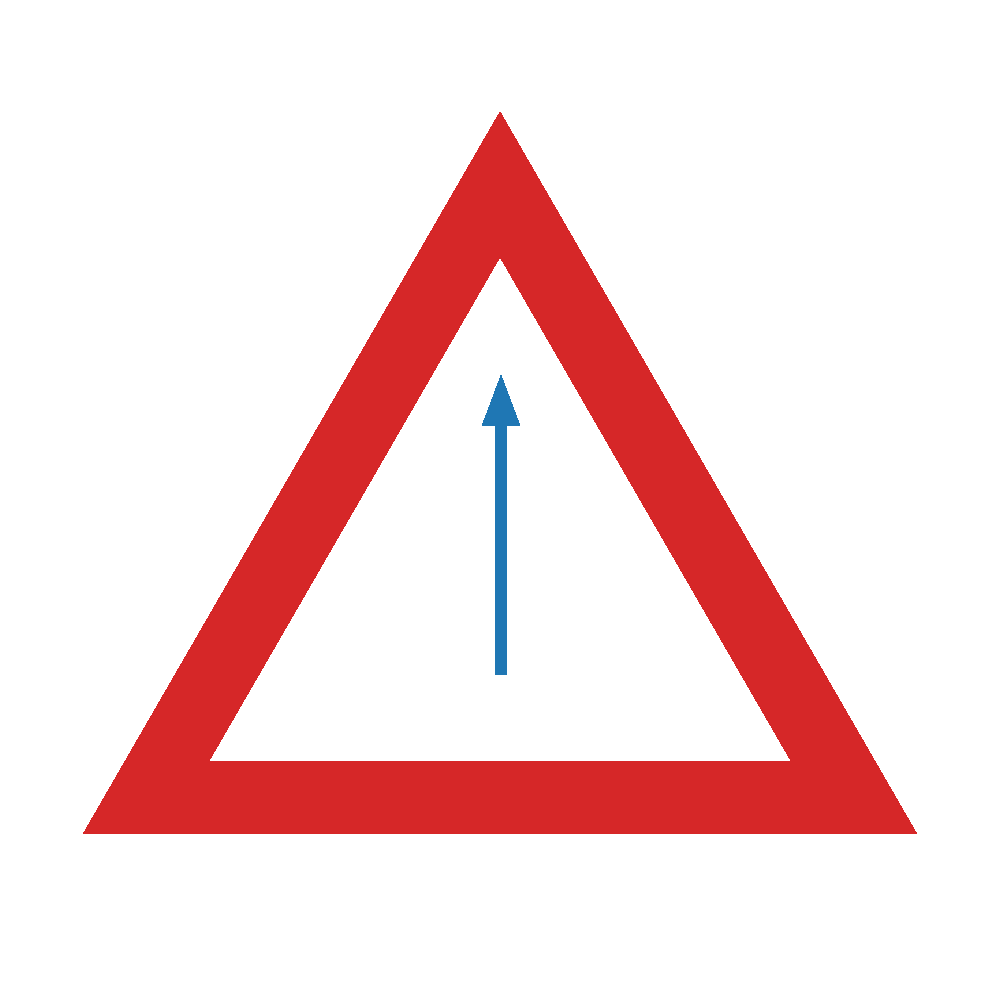
\includegraphics[width=0.30\textwidth]{./figures/hollow-triangle-constant-vector-potential.pdf}
      \end{figure}

      \vspace{-15mm}
      \begin{figure}
        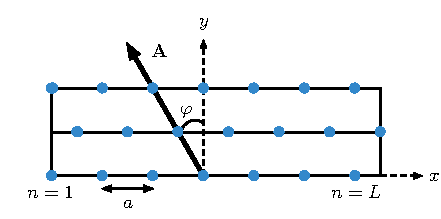
\includegraphics[width=0.3\textwidth]{./figures/triangular-lattice-finite-width-ribbon.pdf}
      \end{figure}

      \pause

      \begin{figure}
        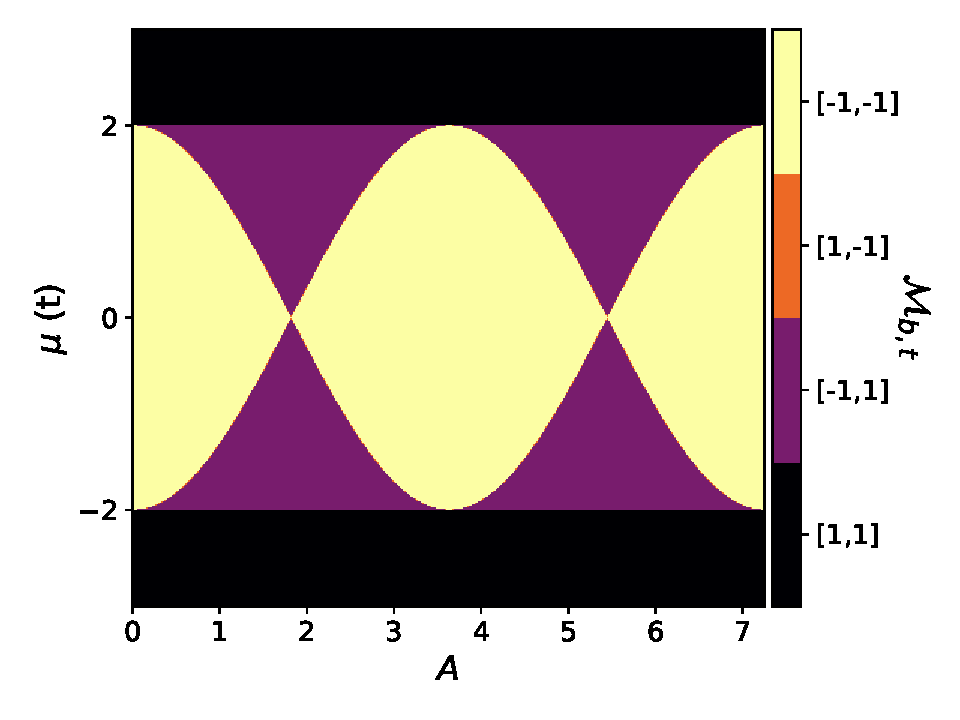
\includegraphics[width=0.4\textwidth]{./figures/topological-phase-diagram-1pi3-w-1.pdf} \\
        \hspace{-10mm}
        \pause
        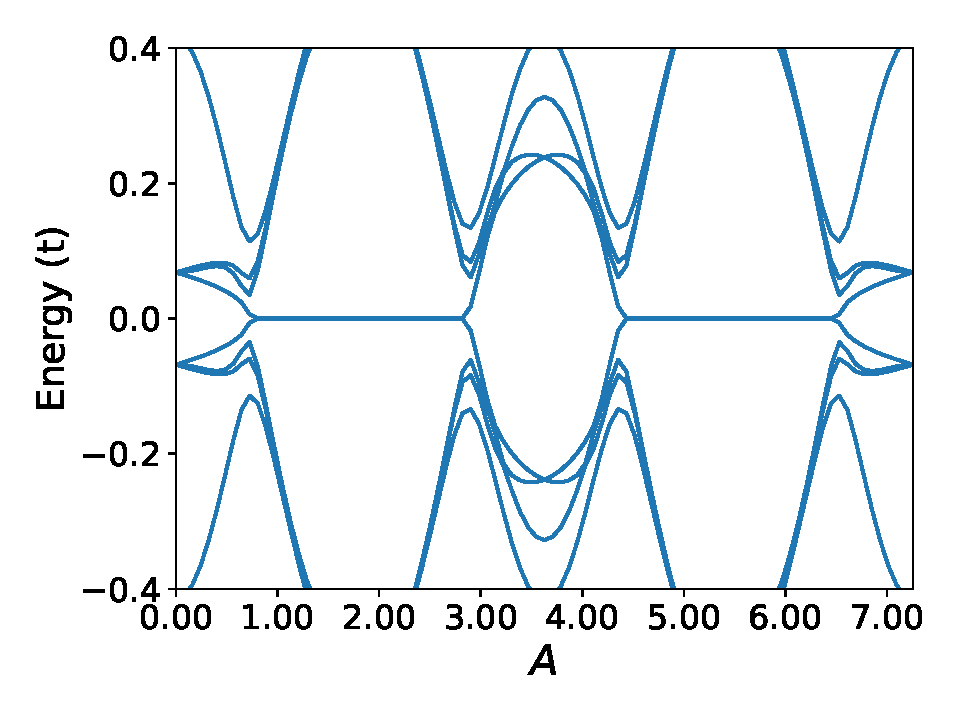
\includegraphics[width=0.34\textwidth]{./figures/spectral-flow-nr-50-w-1-mu-1_6.pdf}
      \end{figure}
    \end{multicols}

  \end{frame}

  \begin{frame}
    \frametitle{Rotating MZMs on a Triangular Chain (W=1)}

    \begin{figure}
      \begin{tikzpicture}
        \node[inner sep=0pt] (figure) at (-2.8,0){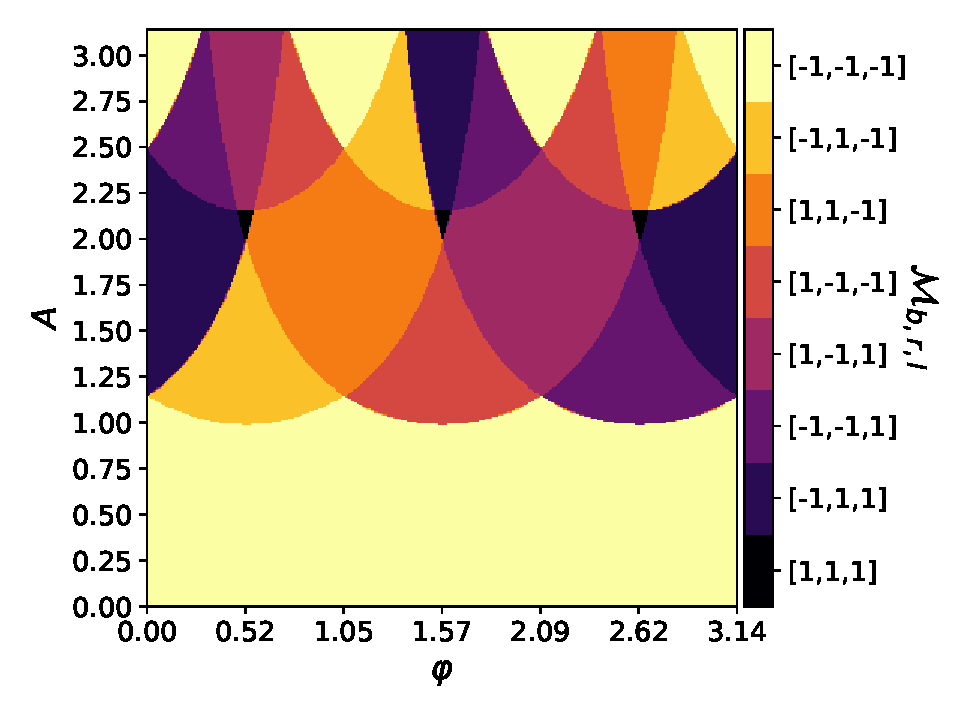
\includegraphics[width=0.4\textwidth]{./figures/topological-phase-diagram-w-1-mu-p1_1000.pdf}};
        \pause
        \draw[line width=0.3mm, green] (-4.62,1) -- (-1.4,1);
        \node[inner sep=0pt] (figure2) at (2.8,0){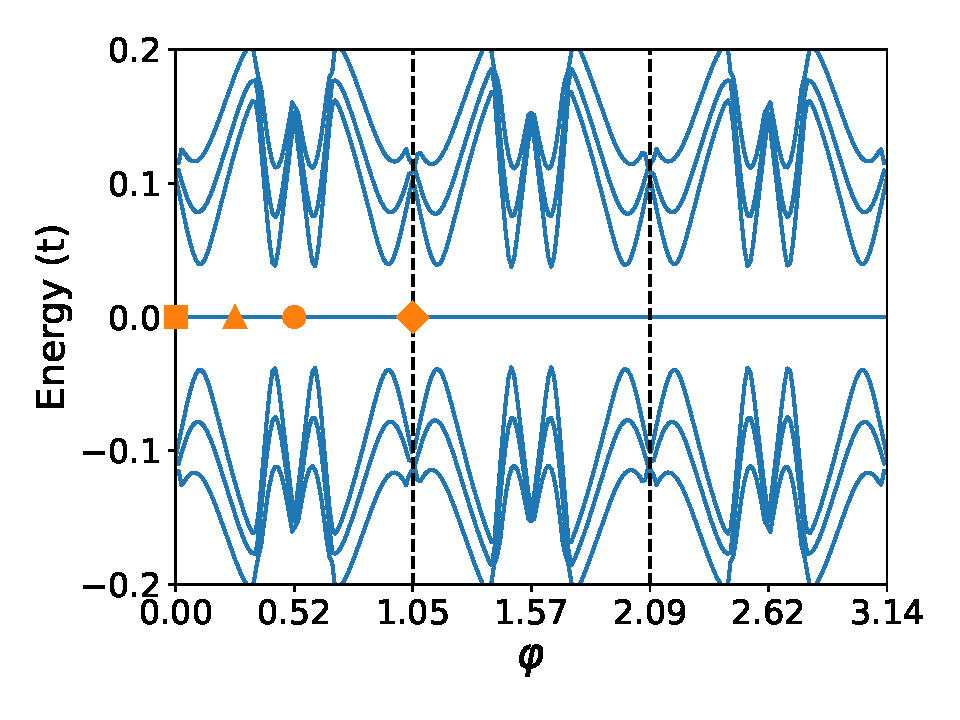
\includegraphics[width=0.4\textwidth]{./figures/spectral-flow-rotation-constant-vector-nr-50-w-1-mu-1_1.pdf}};
        \node[inner sep=0pt] (caption) at (0,-2.0) {\footnotesize $L=50$, $W=1$, $\mu=1.1$, $A=2.35$};
        \onslide<1->
      \end{tikzpicture}
    \end{figure}
    \pause
    \begin{figure}
      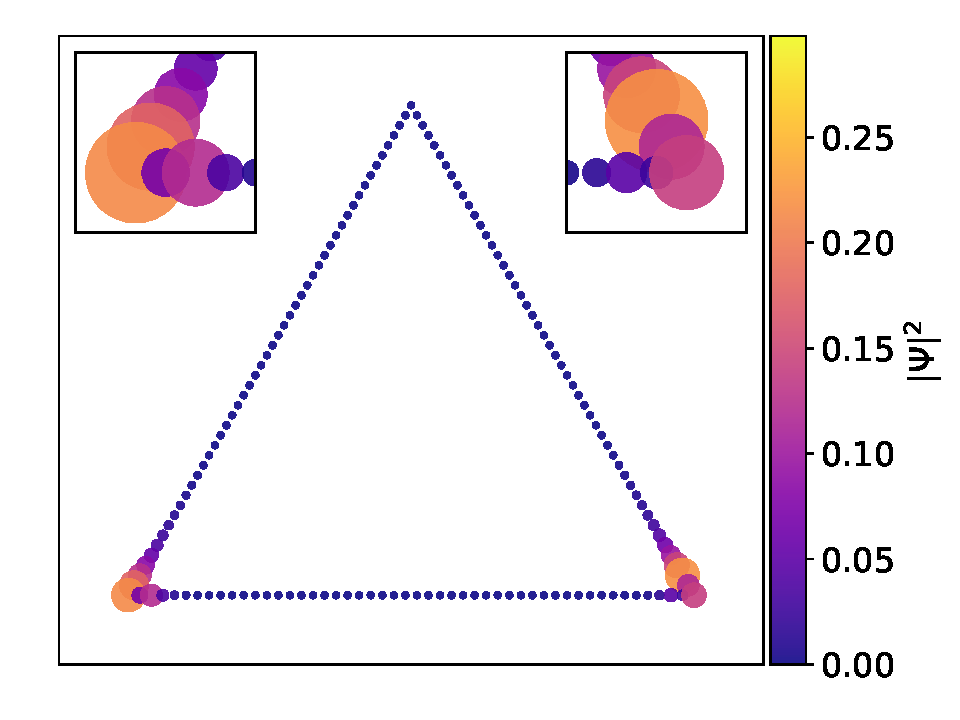
\includegraphics[height=80pt]{./figures/GS-T-Square.pdf}\hspace{-25pt}
      \pause
      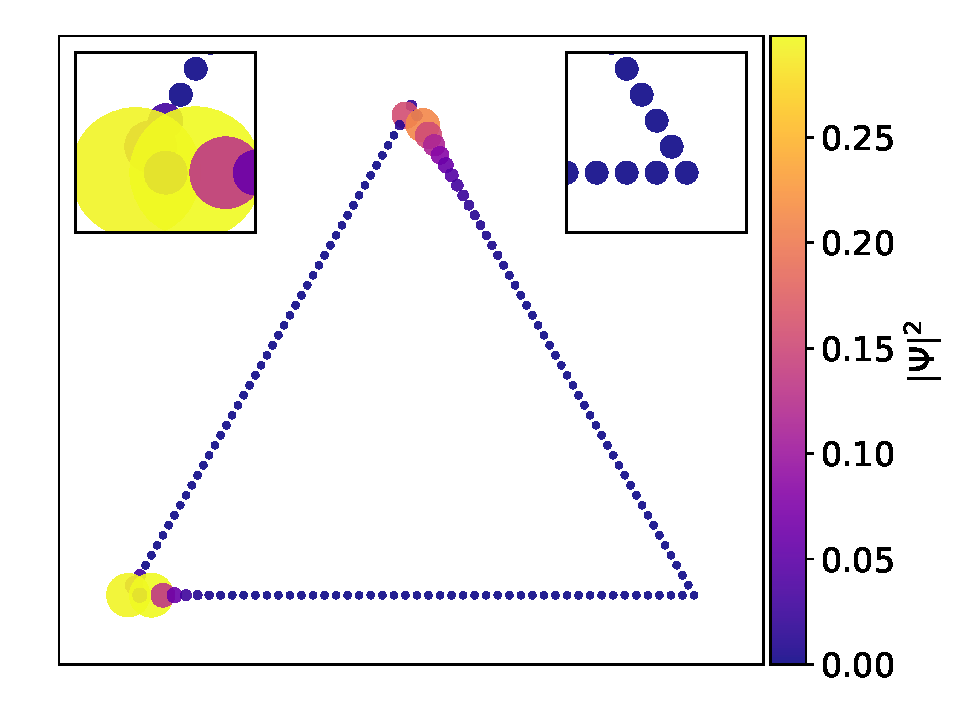
\includegraphics[height=80pt]{./figures/GS-T-Triangle.pdf}\hspace{-25pt}
      \pause
      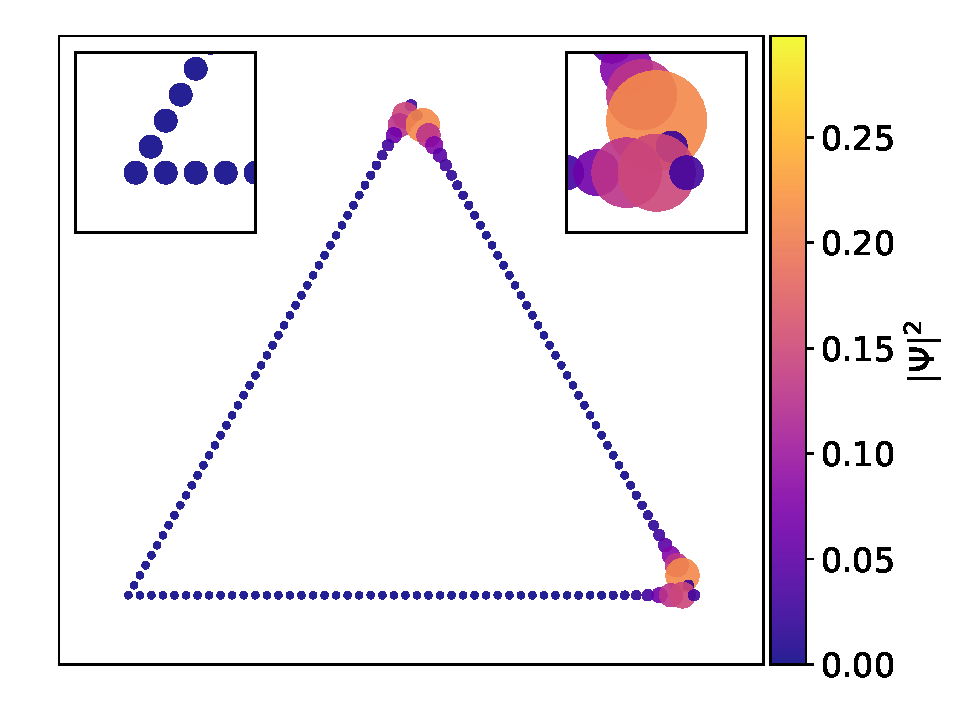
\includegraphics[height=80pt]{./figures/GS-T-Circle.pdf}\hspace{-25pt}
      \pause
      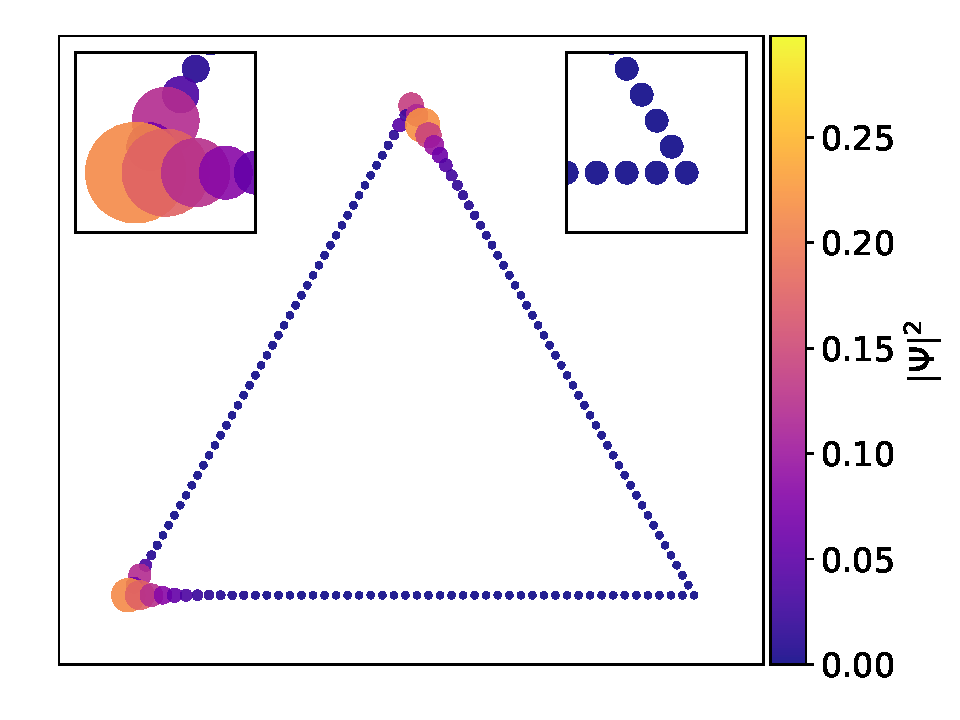
\includegraphics[height=80pt]{./figures/GS-T-Diamond.pdf}
    \end{figure}
  \end{frame}

  \begin{frame}
    \frametitle{Rotating MZMs on a Hollow Triangle (W=3)}

    \begin{figure}
      \begin{tikzpicture}
        \node[inner sep=0pt] (figure) at (-4.4,0.0){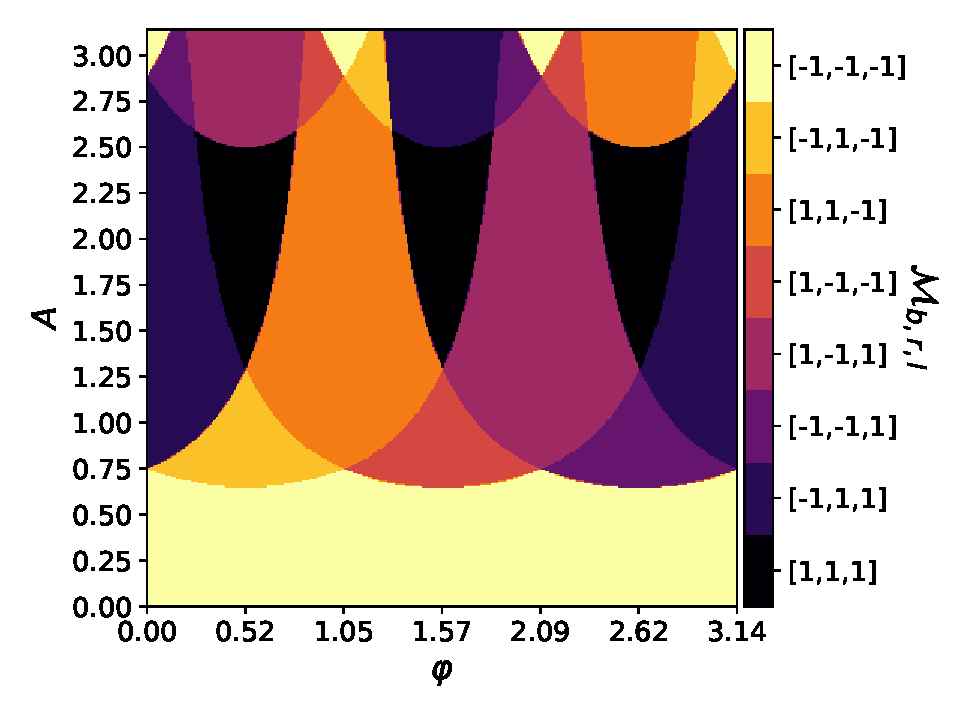
\includegraphics[width=0.33\textwidth]{./figures/topological-phase-diagram-w-3-mu-p1_6000.pdf}};
        \node[inner sep=0pt] (figure2) at (0,0){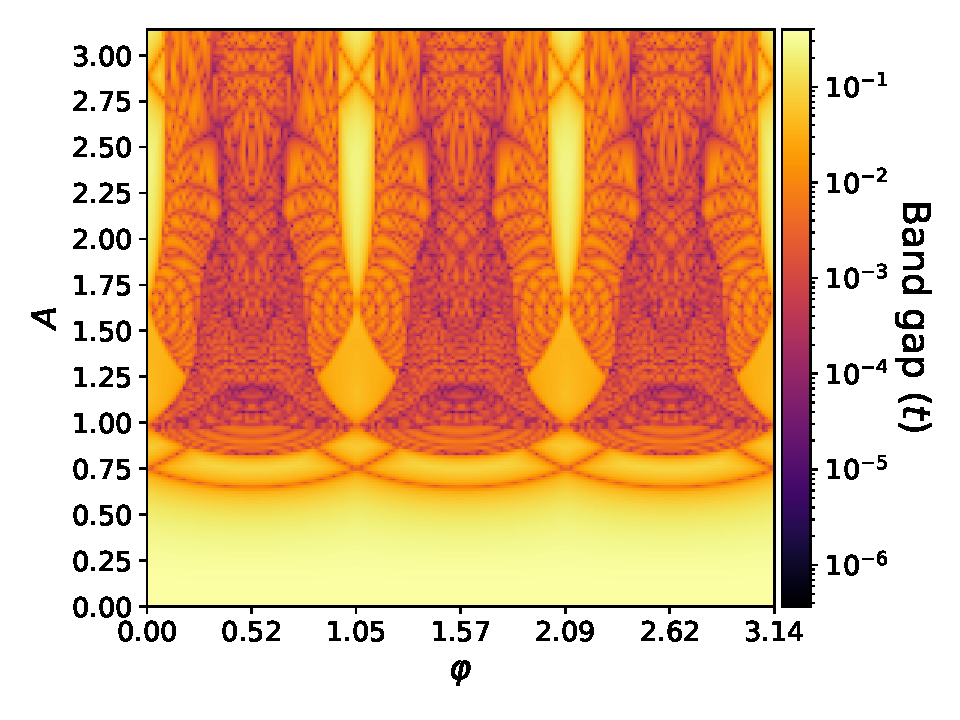
\includegraphics[width=0.33\textwidth]{./figures/band-gap-rotation-w-3-mu-p1_6000.pdf}};
        \pause
        \draw[line width = 0.2mm, green] (-5.9,-0.43) -- (-5.45,-0.51);
        \draw[line width = 0.2mm, green] (-5.45,-0.51) -- (-5.01,-0.43);
        \draw[line width = 0.2mm, green] (-5.01,-0.43) -- (-4.56,-0.51);
        \draw[line width = 0.2mm, green] (-4.56,-0.51) -- (-4.13,-0.43);
        \draw[line width = 0.2mm, green] (-4.13,-0.43) -- (-3.68,-0.51);
        \draw[line width = 0.2mm, green] (-3.68,-0.51) -- (-3.25,-0.43);
        \draw[line width = 0.2mm, green] (-1.50,-0.43) -- (-1.05,-0.51);
        \draw[line width = 0.2mm, green] (-1.05,-0.51) -- (-0.56,-0.43);
        \draw[line width = 0.2mm, green] (-0.56,-0.43) -- (-0.07,-0.51);
        \draw[line width = 0.2mm, green] (-0.07,-0.51) -- (0.39,-0.43);
        \draw[line width = 0.2mm, green] (0.39,-0.43) -- (0.86,-0.51);
        \draw[line width = 0.2mm, green] (0.86,-0.51) -- (1.32,-0.43);
        \node[inner sep=0pt] (figure3) at (4.4,0){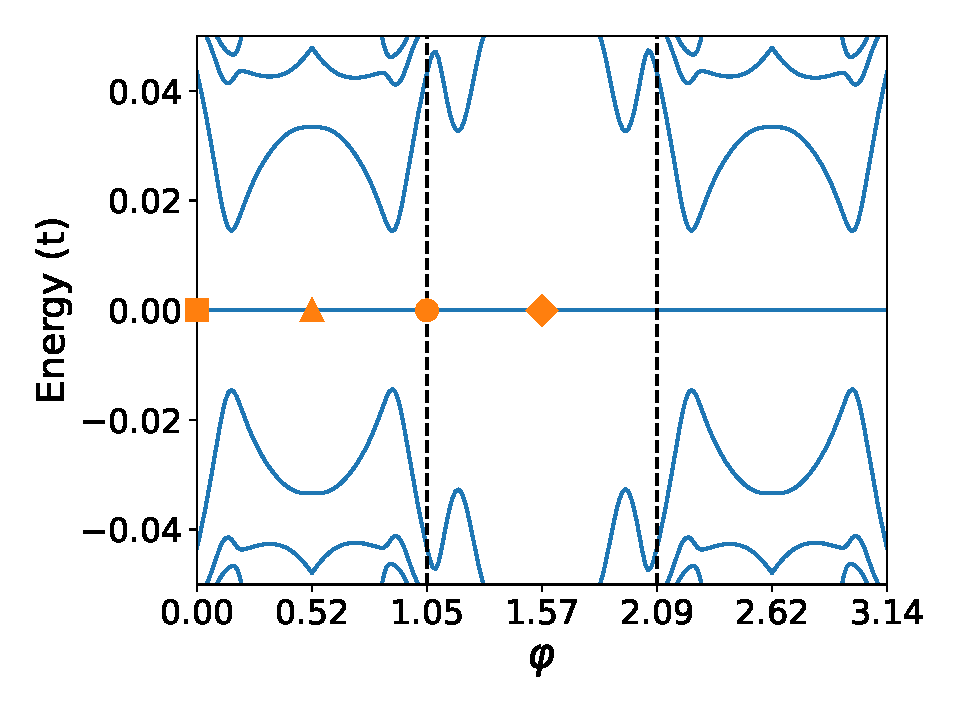
\includegraphics[width=0.33\textwidth]{./figures/spectral-flow-rotation-nr-80-w-3-mu-p1_6000.pdf}};
        \node[inner sep=0pt] (caption) at (0,-2.0) {\footnotesize $L=80$, $W=3$, $\mu=1.6$, $(A,\varphi) = (0.83,0) \rightarrow (0.77,\pi/6) \rightarrow (0.83,\pi/3) \rightarrow \dots$};
        \onslide<1->
      \end{tikzpicture}
    \end{figure}

    \pause
    \begin{figure}
      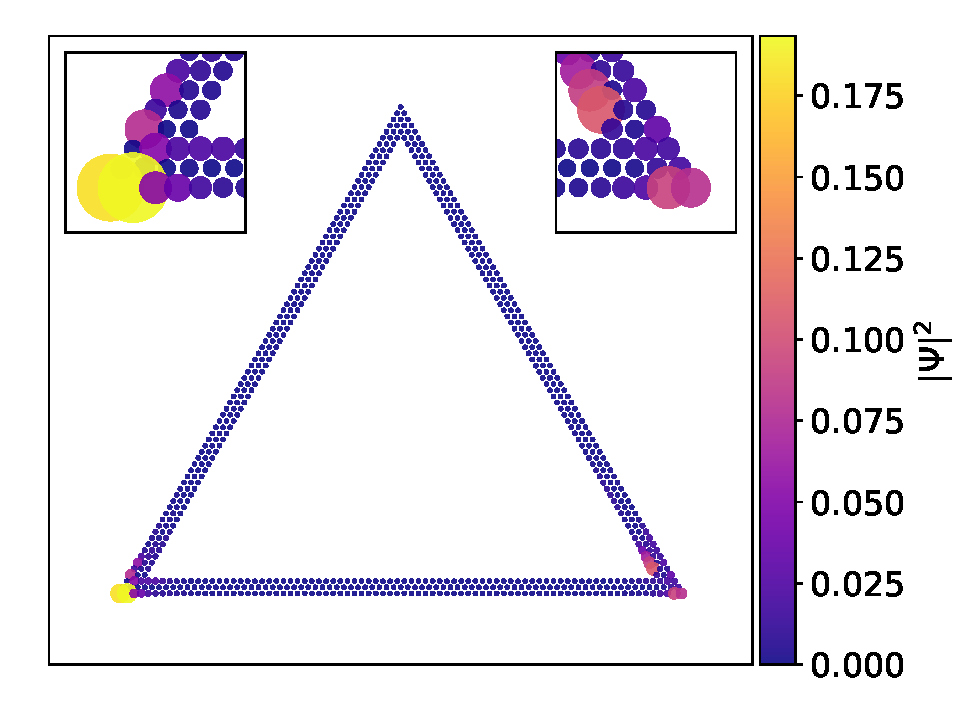
\includegraphics[height=80pt]{./figures/GS-T-Square-w-3.pdf}\hspace{-26pt}
      \pause
      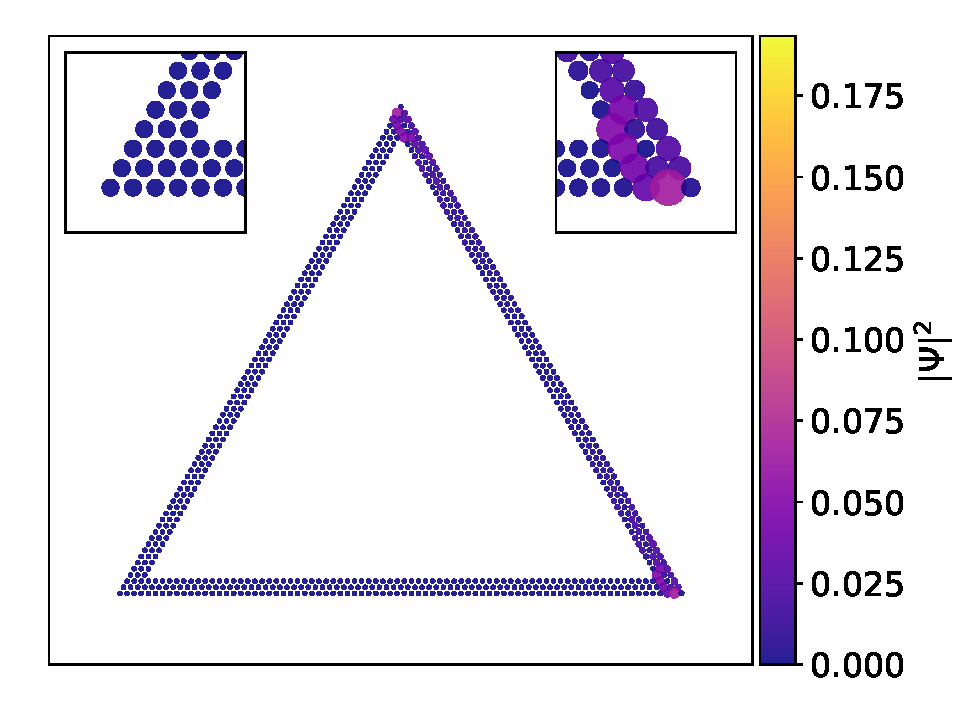
\includegraphics[height=80pt]{./figures/GS-T-Triangle-w-3.pdf}\hspace{-26pt}
      \pause
      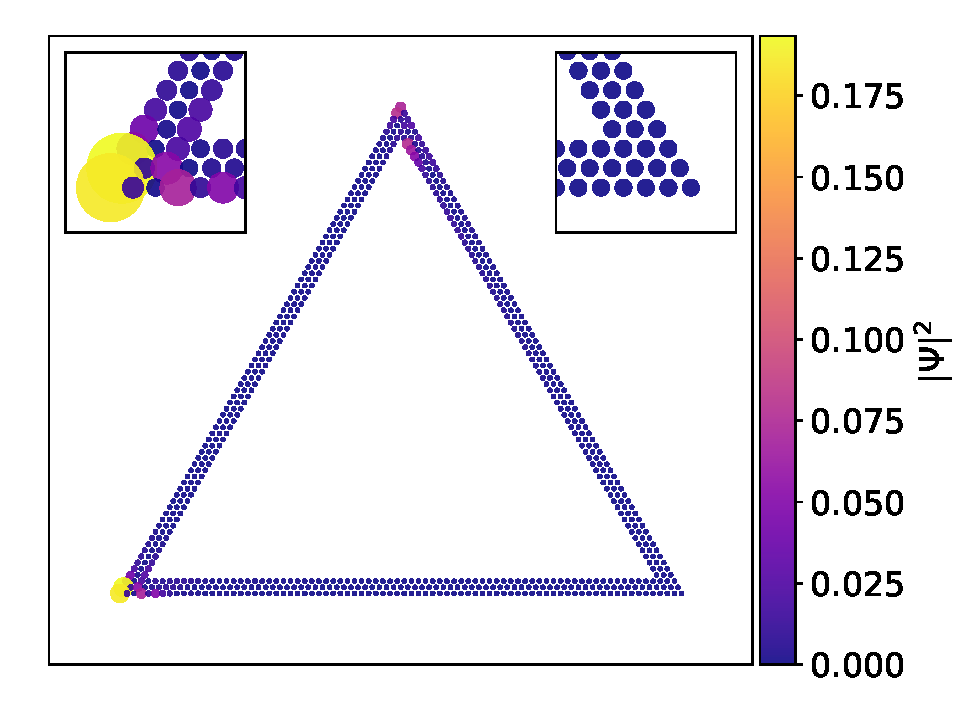
\includegraphics[height=80pt]{./figures/GS-T-Circle-w-3.pdf}\hspace{-26pt}
      \pause
      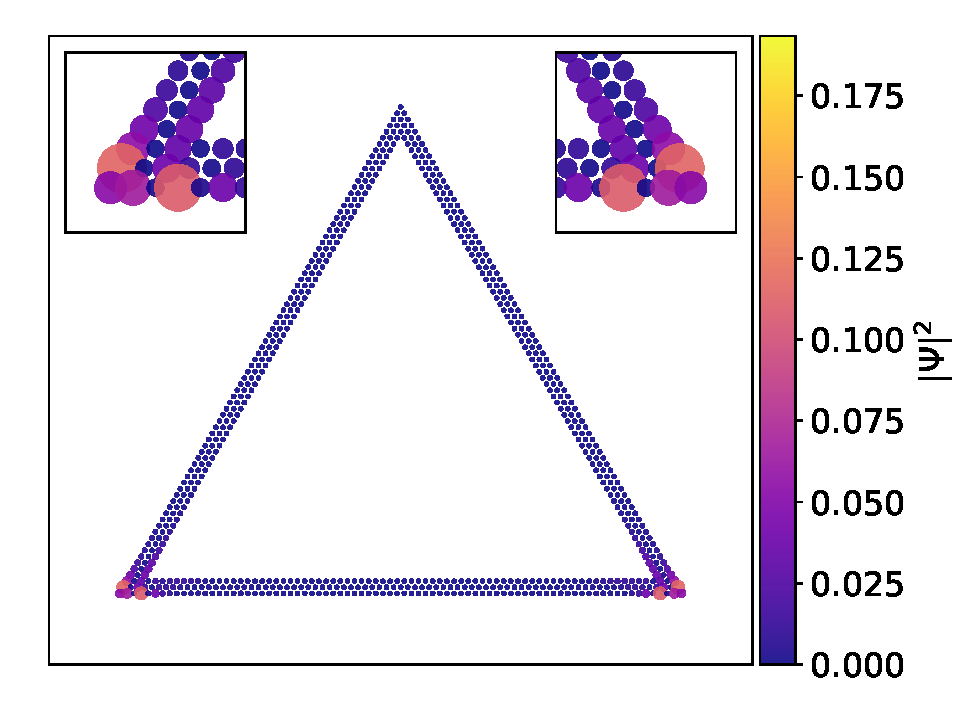
\includegraphics[height=80pt]{./figures/GS-T-Diamond-w-3.pdf}
    \end{figure}


  \end{frame}

  \section{\BR}
  \begin{frame}
    \frametitle{Braiding Two of Four MZMs}
    \begin{figure}
      \begin{tikzpicture}
        \node[inner sep=0pt] (figure) at (0,0) {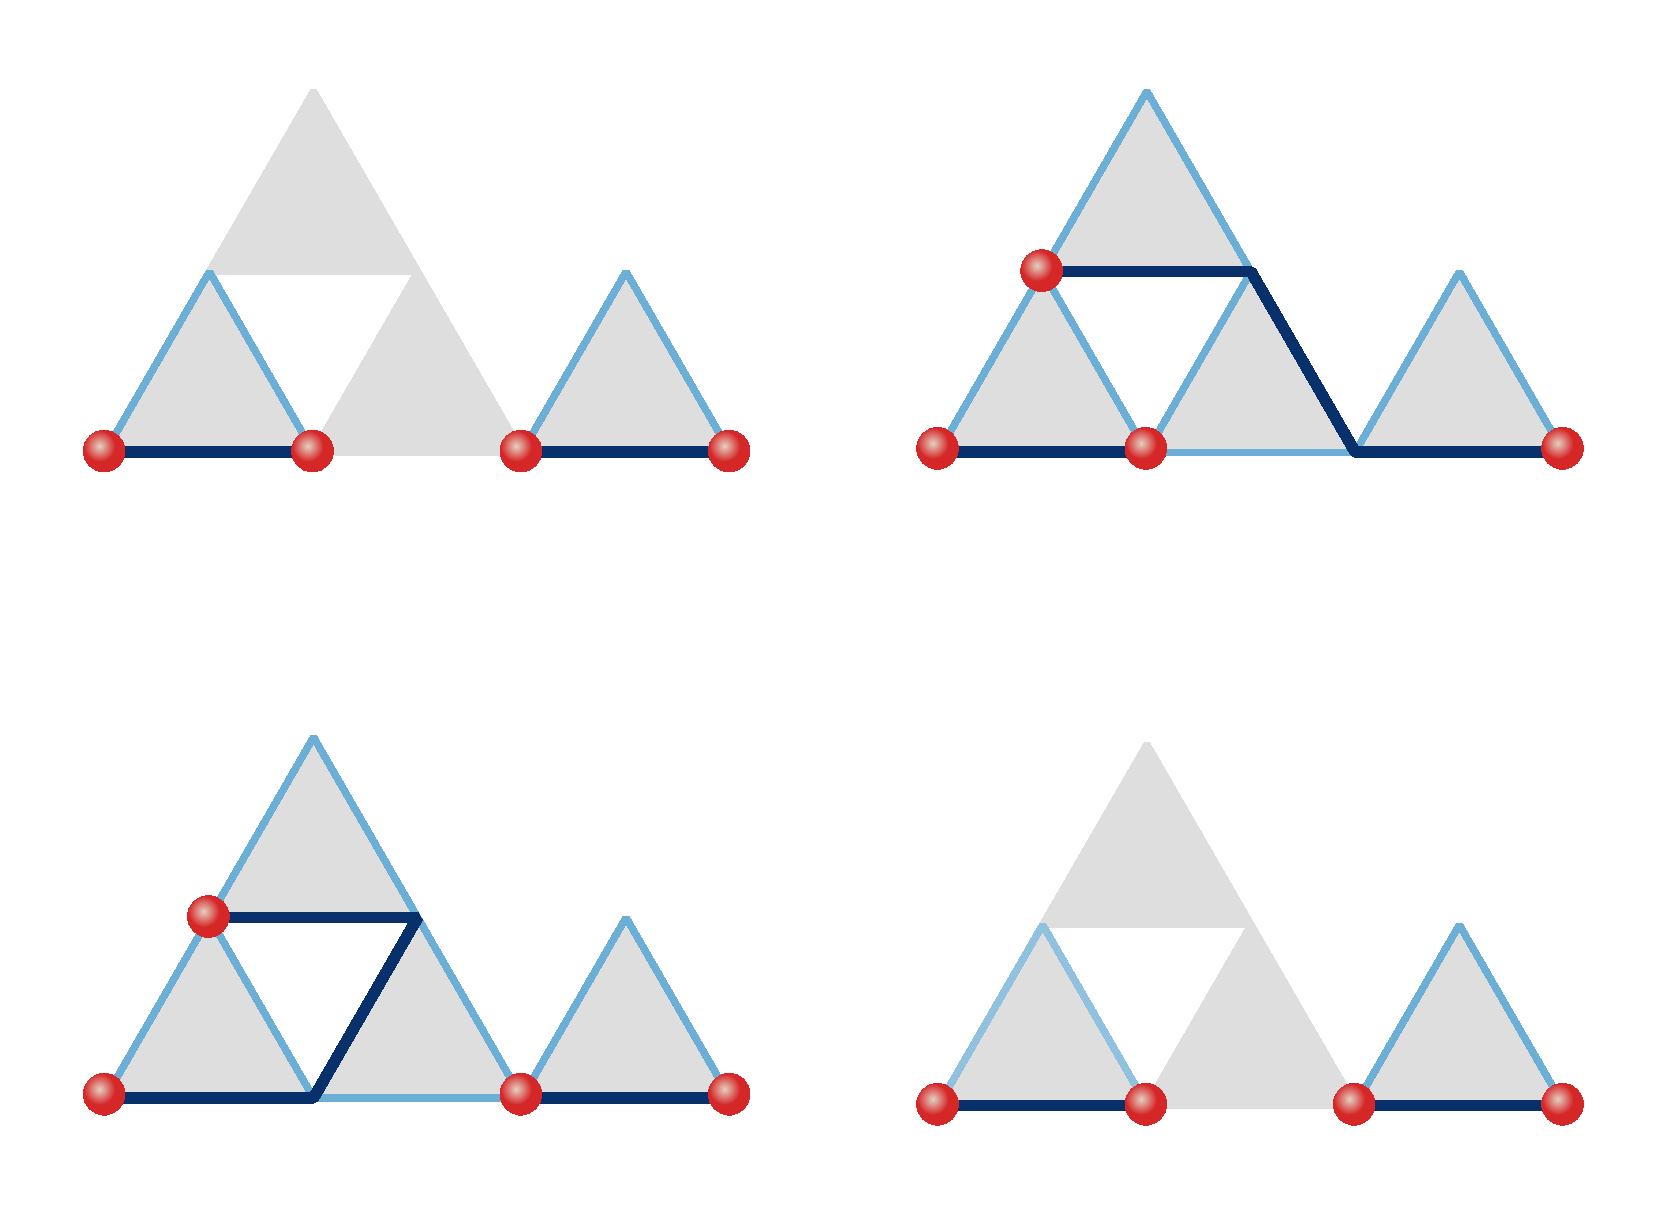
\includegraphics[width=0.8\textwidth]{./figures/4-mf-swap-2-3.pdf}};

         \node[inner sep=0pt] (gamma1) at (-4.3,0.75) {$\gamma_1$};
         \node[inner sep=0pt] (gamma2) at (-3.0,0.75) {$\gamma_2$};
         \node[inner sep=0pt] (gamma3) at (-1.7,0.75) {$\gamma_3$};
         \node[inner sep=0pt] (gamma4) at (-0.4,0.75) {$\gamma_4$};

         \node[inner sep=0pt] (gamma1) at (0.90,0.75) {$\gamma_1$};
         \node[inner sep=0pt] (gamma2) at (2.20,0.75) {$\gamma_2$};
         \node[inner sep=0pt] (gamma3) at (0.90,2.25) {$\gamma_3$};
         \node[inner sep=0pt] (gamma4) at (4.80,0.75) {$\gamma_4$};

h        \node[inner sep=0pt] (gamma1) at (-4.3,-3.35) {$\gamma_1$};
         \node[inner sep=0pt] (gamma3) at (-4.3,-1.80) {$\gamma_3$};
         \node[inner sep=0pt] (gamma2) at (-1.7,-3.35) {$\gamma_2$};
         \node[inner sep=0pt] (gamma4) at (-0.4,-3.35) {$\gamma_4$};

         \node[inner sep=0pt] (gamma1) at (0.90,-3.35) {$\gamma_1$};
         \node[inner sep=0pt] (gamma3) at (2.20,-3.35) {$\gamma_3$};
         \node[inner sep=0pt] (gamma2) at (3.50,-3.35) {$\gamma_2$};
         \node[inner sep=0pt] (gamma4) at (4.80,-3.35) {$\gamma_4$};

      \end{tikzpicture}
    \end{figure}
  \end{frame}

  \section{\CO}
  \begin{frame}
    \frametitle{Summary}

    \begin{itemize}
      \item Introduction of Peierls phase allows for a minimal Kitaev triangle, reducing fermionic sites down to 3.
      \item Vector potential field and its rotation allows additional tunability of topology.
      \item MZMs can be hosted and braided on a network of triangular islands.
    \end{itemize}
  \end{frame}

  \appendix

  \begin{frame}
  \frametitle{Majorana fermion notation and coupling isolations}
    The complex fermion operator can be written as a superposition of two Majorana fermions $c_j = \frac{1}{2} (a_j + i b_j)$.
    Due to the nature of Majorana fermions, $a^{\dagger}_j = a_j$, the creation operator is $\cc_j = \frac{1}{2} (a_j - i b_j)$.
    \begin{align*}
      H = -\dfrac{i\mu}{2} \sum_j a_j b_j - \dfrac{i}{2} \sum_{\langle jl\rangle} [&(t\sin\phi_{jl}-\de\sin\theta_{jl}) a_l a_j + (t\sin\phi_{jl}+\de\sin\theta_{jl}) b_l b_j \nonumber \\
      +&(t\cos\phi_{jl}-\de\cos\theta_{jl}) a_l b_j - (t\cos\phi_{jl}+\de\cos\theta_{jl}) b_l a_j].
    \end{align*}
    \begin{align}
      &(t \sin\phi_{jl} - \de \sin\theta_{jl}) a_l a_j, \\
      &(t \sin\phi_{jl} + \de \sin\theta_{jl}) b_l b_j, \\
      &(t \cos\phi_{jl} + \de \cos\theta_{jl}) a_l b_j, \\
      &(t \cos\phi_{jl} - \de \cos\theta_{jl}) b_l a_j
    \end{align}
  \end{frame}

  \begin{frame}
    \frametitle{Braiding MZM in a Small Network of Triangles}
    \begin{figure}
      \subfloat{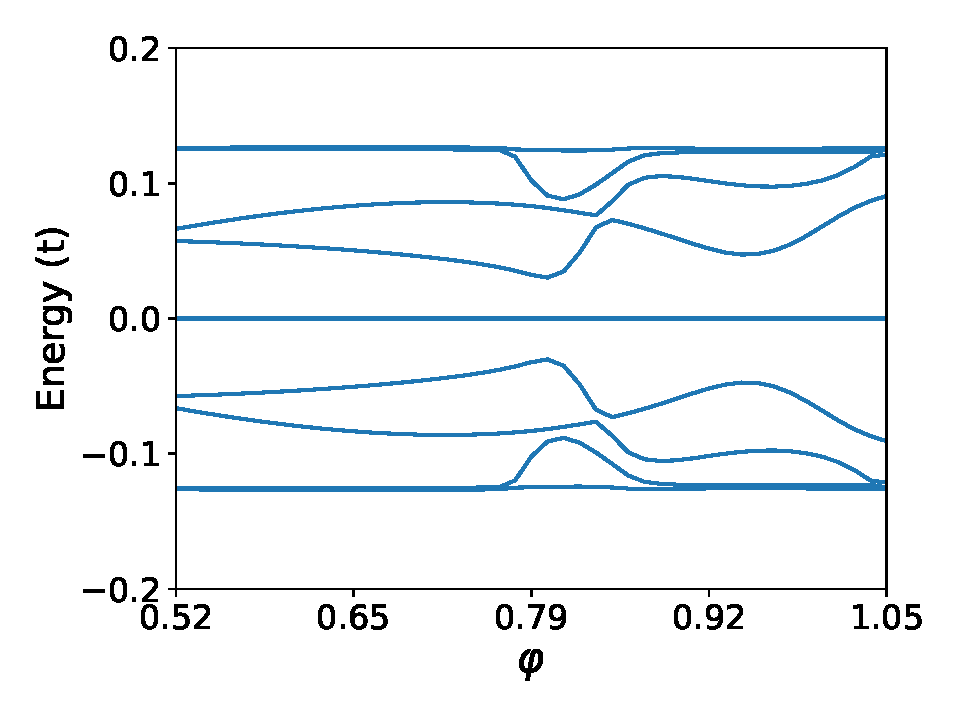
\includegraphics[width=0.33\textwidth]{./figures/supp/spectral-flow-braiding.pdf}} \\
      \subfloat{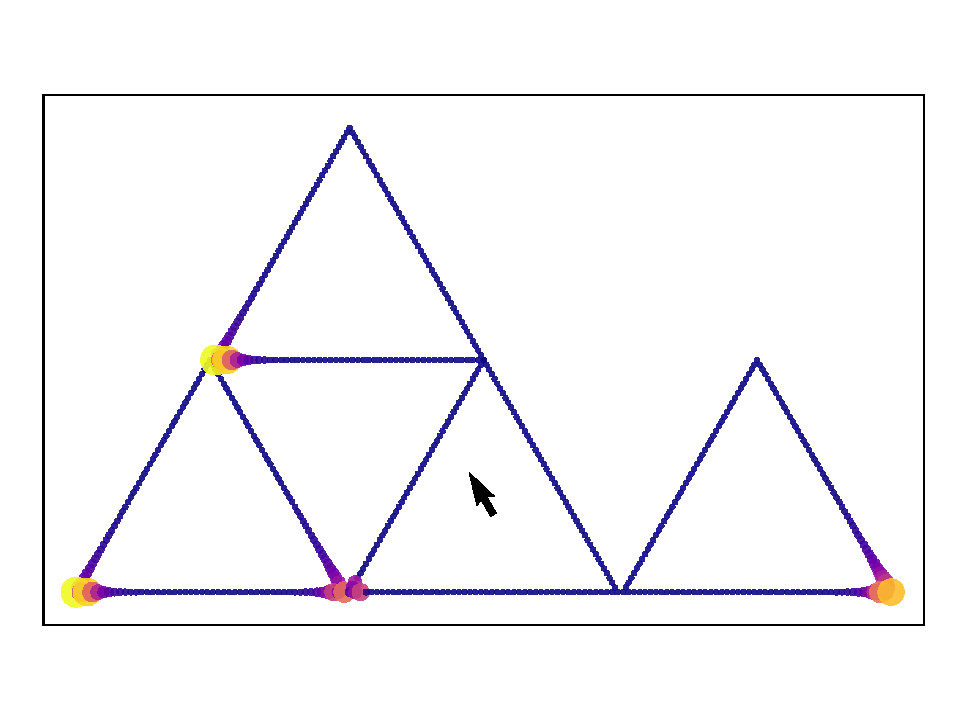
\includegraphics[width=0.25\textwidth]{./figures/supp/GS-T-0_5236.pdf}}
      \subfloat{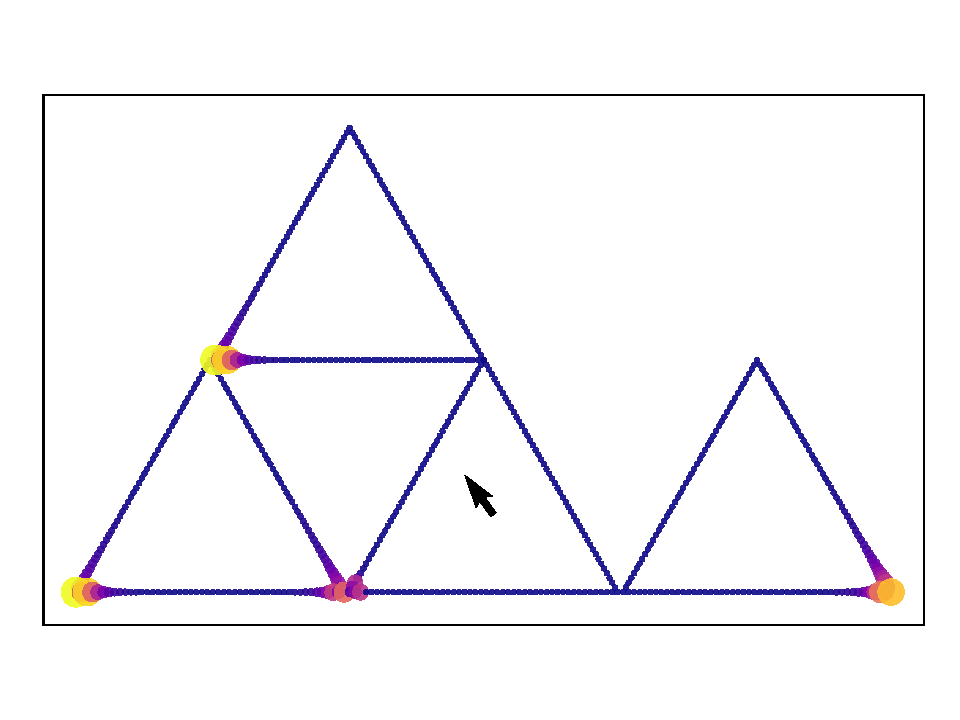
\includegraphics[width=0.25\textwidth]{./figures/supp/GS-T-0_6283.pdf}}
      \subfloat{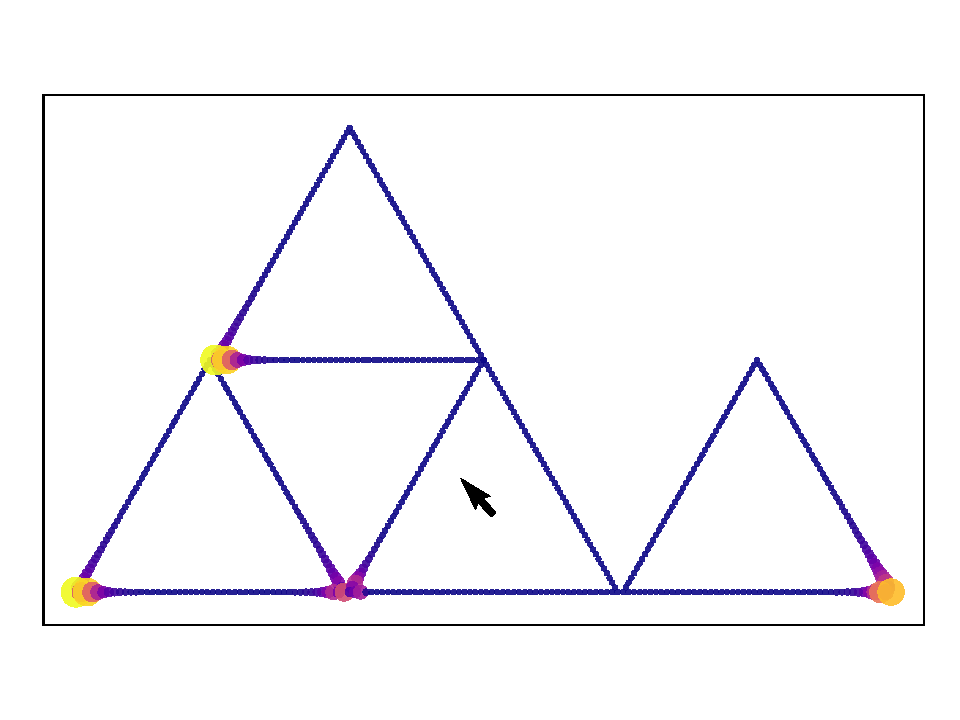
\includegraphics[width=0.25\textwidth]{./figures/supp/GS-T-0_7330.pdf}} \\
      \vspace{-03mm}
      \subfloat{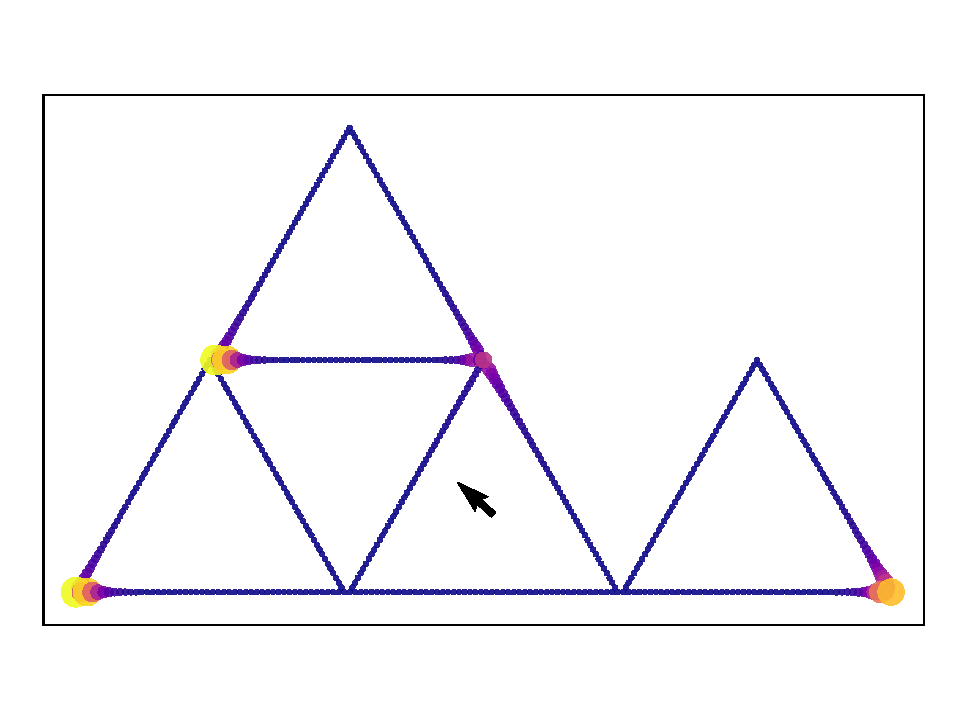
\includegraphics[width=0.25\textwidth]{./figures/supp/GS-T-0_8378.pdf}}
      \subfloat{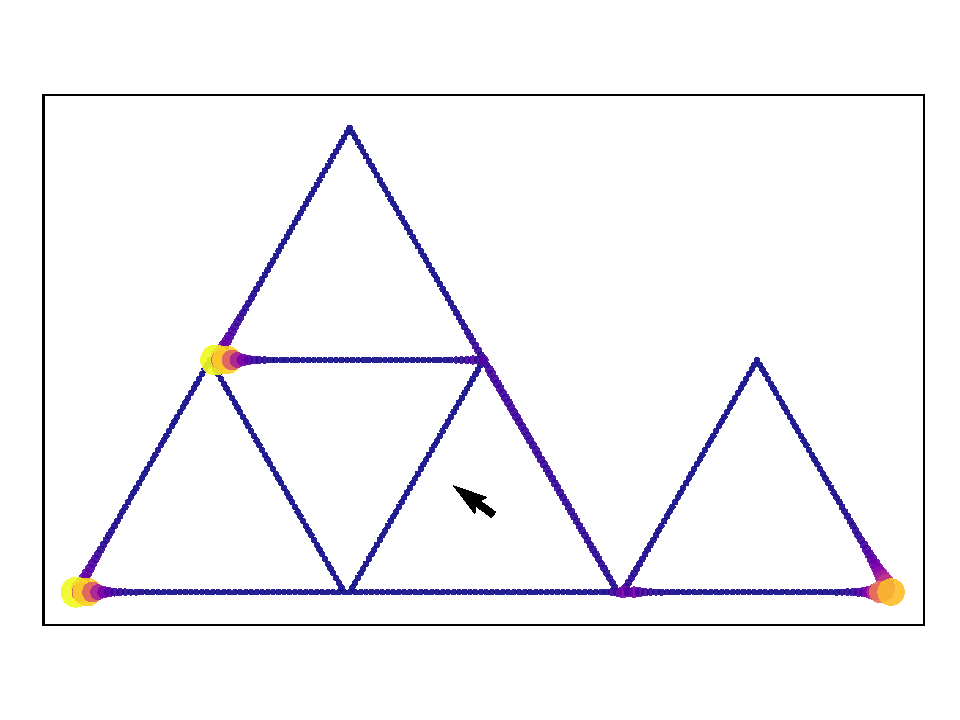
\includegraphics[width=0.25\textwidth]{./figures/supp/GS-T-0_9425.pdf}}
      \subfloat{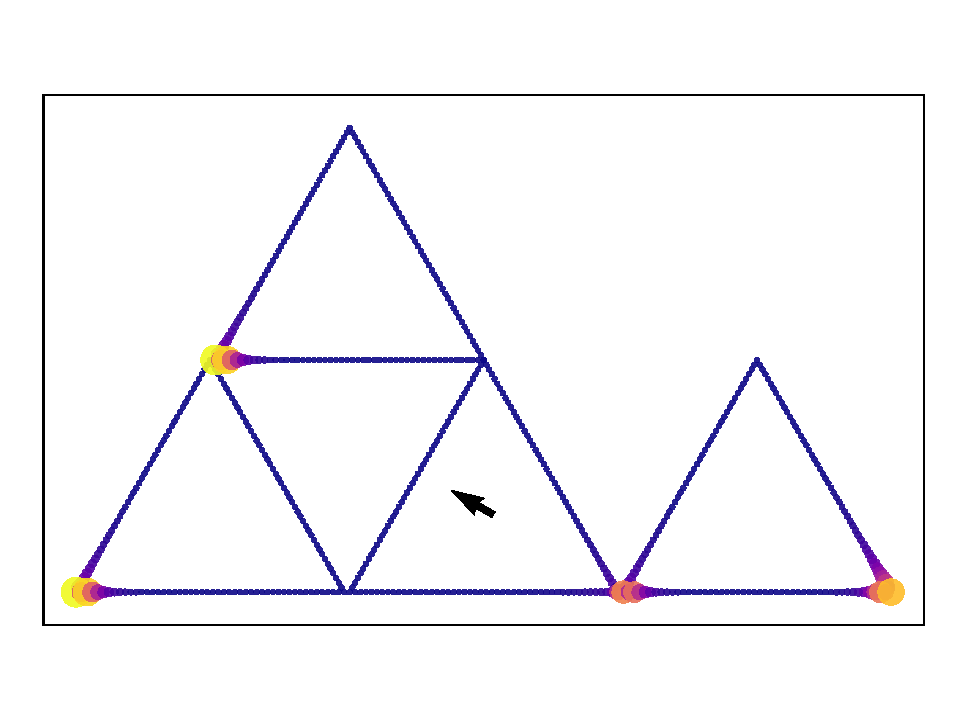
\includegraphics[width=0.25\textwidth]{./figures/supp/GS-T-1_0472.pdf}}
    \end{figure}
  \end{frame}

  \begin{frame}
    \frametitle{Braiding MZM in a Small Network of Triangles}
    \begin{multicols}{3}
      \vspace{10em}
      \begin{figure}
        \subfloat{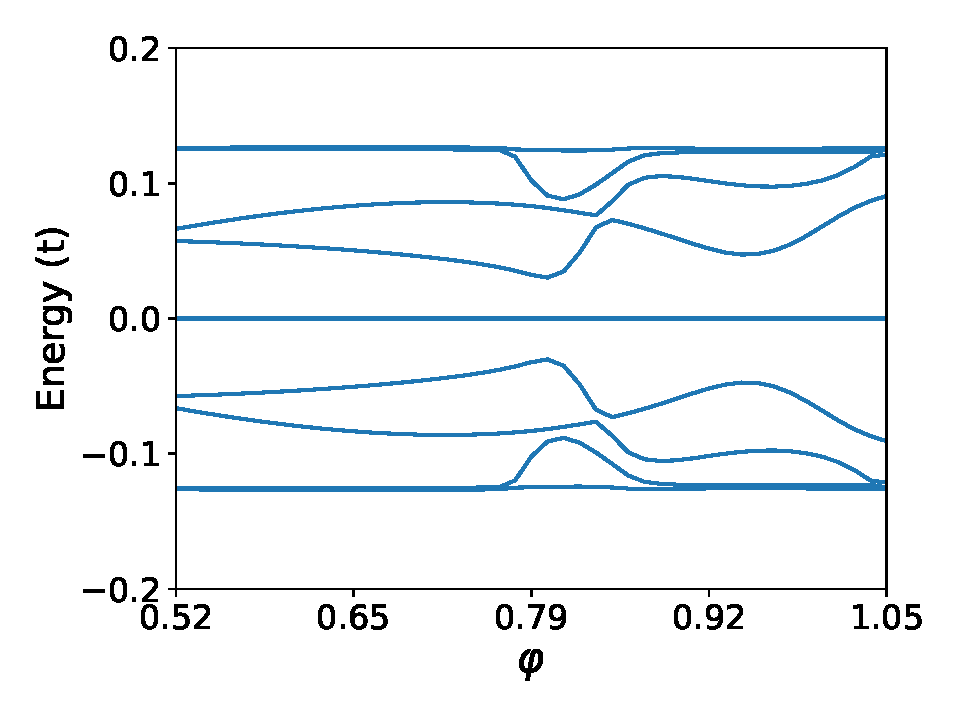
\includegraphics[width=0.3\textwidth]{./figures/supp/spectral-flow-braiding.pdf}}
      \end{figure}
      \vspace{10em}
      \begin{figure}
        \subfloat{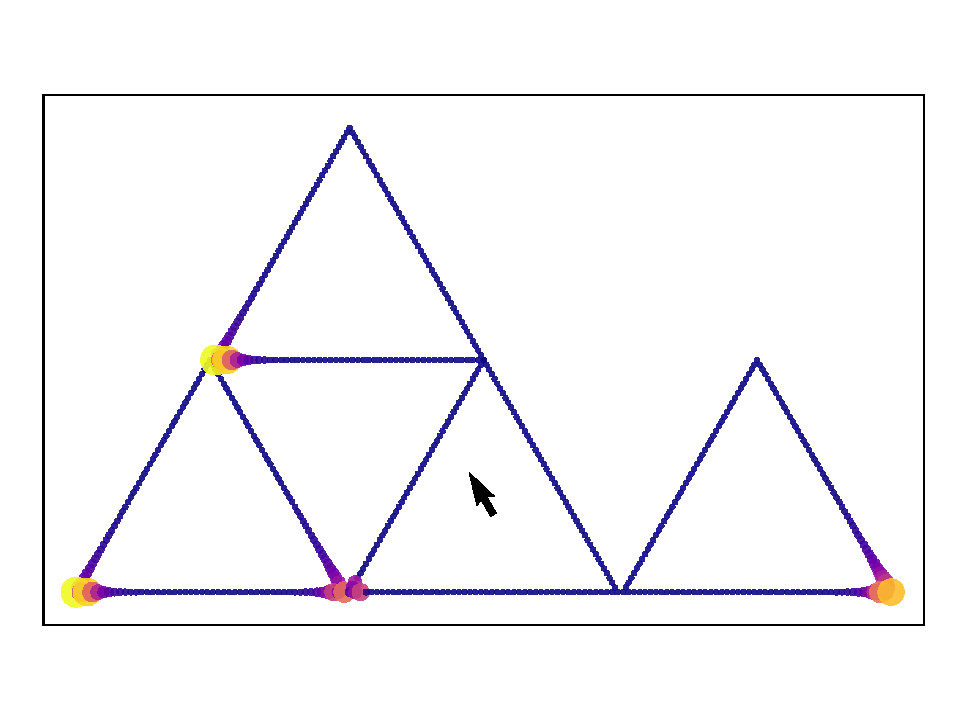
\includegraphics[width=0.27\textwidth]{./figures/supp/GS-T-0_5236.pdf}} \\
        \vspace{-03mm}
        \subfloat{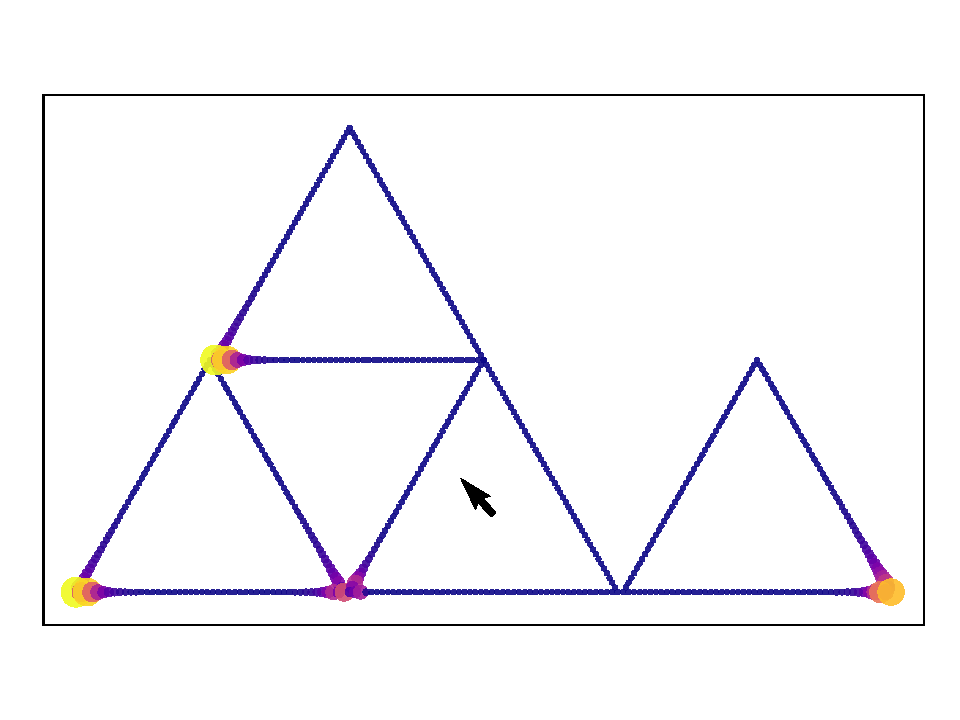
\includegraphics[width=0.27\textwidth]{./figures/supp/GS-T-0_7330.pdf}} \\
        \vspace{-03mm}
        \subfloat{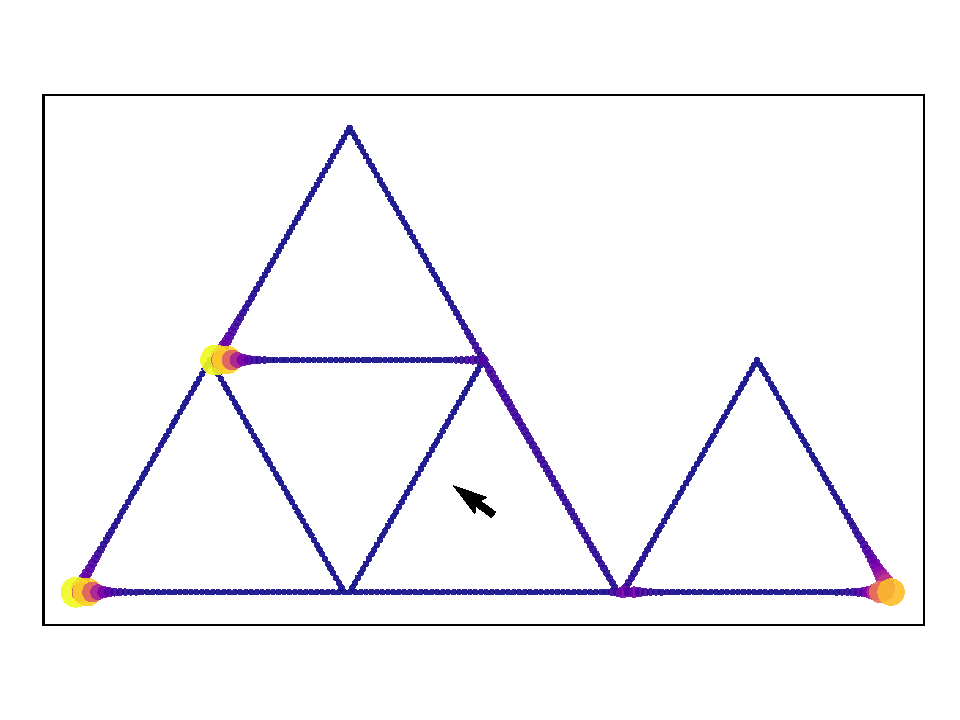
\includegraphics[width=0.27\textwidth]{./figures/supp/GS-T-0_9425.pdf}} \\
      \end{figure}
      \begin{figure}
        \subfloat{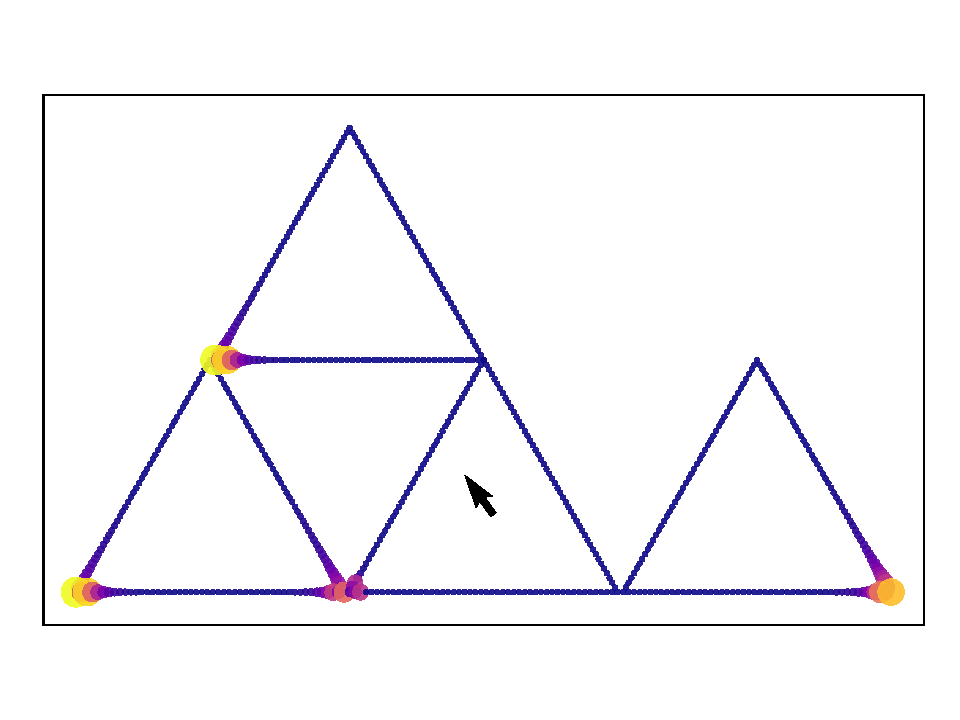
\includegraphics[width=0.27\textwidth]{./figures/supp/GS-T-0_6283.pdf}} \\
        \vspace{-03mm}
        \subfloat{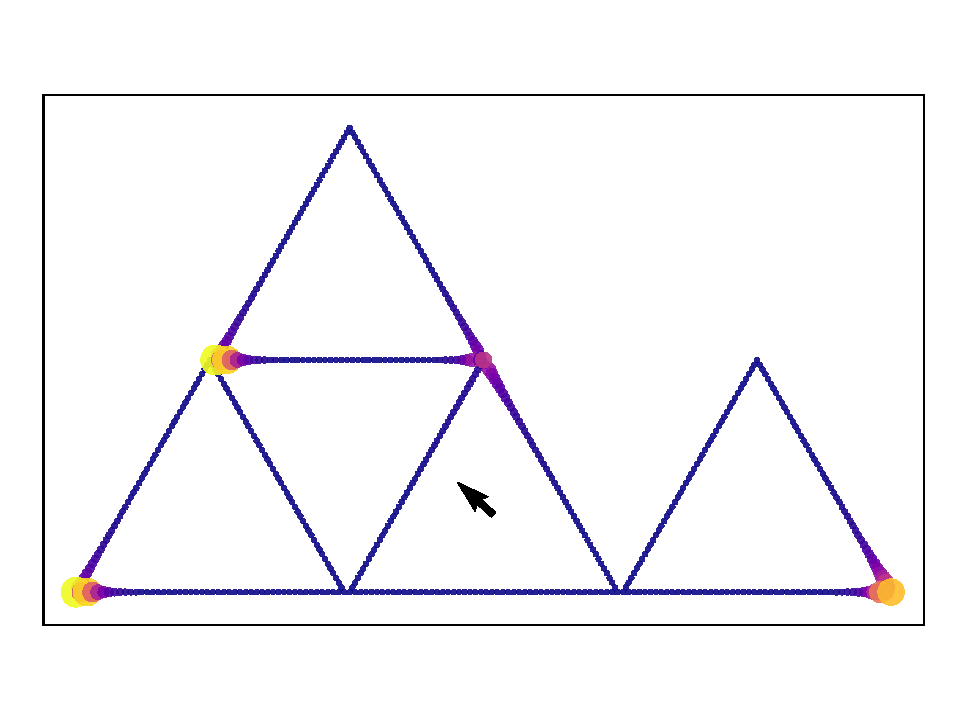
\includegraphics[width=0.27\textwidth]{./figures/supp/GS-T-0_8378.pdf}} \\
        \vspace{-03mm}
        \subfloat{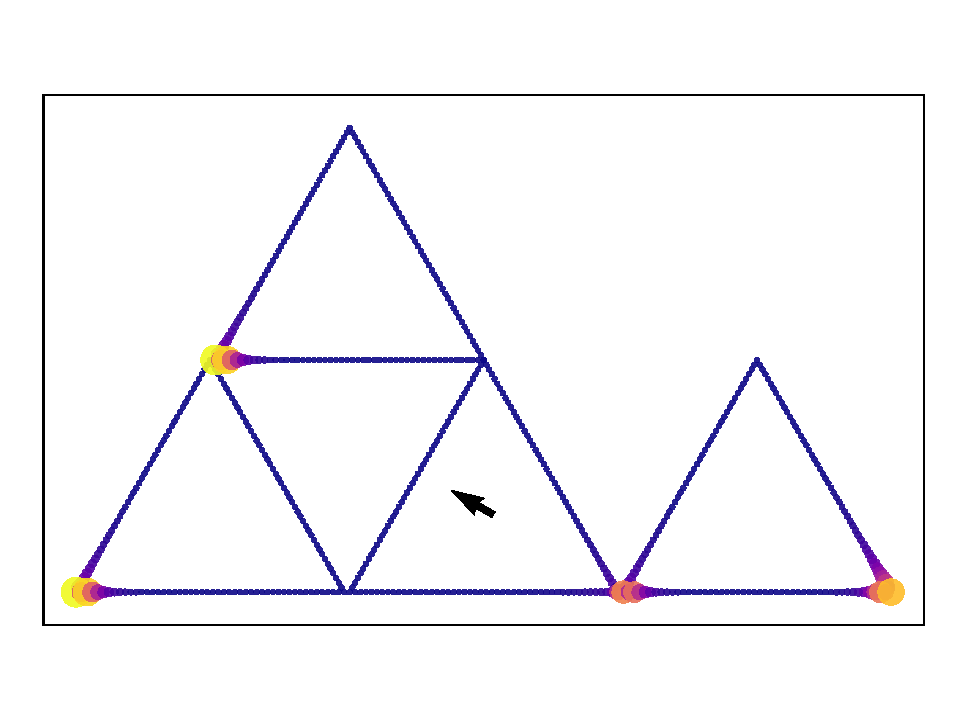
\includegraphics[width=0.27\textwidth]{./figures/supp/GS-T-1_0472.pdf}}
      \end{figure}
    \end{multicols}
  \end{frame}

\end{document}


